%!TEX TS-program = xelatex
%!TEX encoding = UTF-8

\documentclass[mathserif]{ctexbeamer}

\usepackage[orientation=landscape,size=custom,width=16,height=9,scale=0.5,debug]{beamerposter}

\usepackage{amsmath}
\usepackage{mathrsfs}
\usepackage{multicol}

\usetheme{Berlin}
\usecolortheme{spruce}
\usefonttheme{professionalfonts,structurebold}

% \usepackage{beamerthemesplit} // Activate for custom appearance

% \usepackage{fontspec}

% \defaultfontfeatures{Mapping=tex-text}
% \setsansfont{CMU Serif}
\setsansfont{TeX Gyre Heros}
\setCJKsansfont{Noto Sans CJK SC}

\setCJKfamilyfont{emfont}[
	BoldFont=Noto Sans CJK SC Bold
]{Noto Sans CJK SC}
\renewcommand{\em}{\bfseries\sffamily\CJKfamily{emfont}} % 强调

\title{生成函数的一丶进展}
\author{李白天(Elegia)}
\date{2021 年 2 月}

\institute{北京大学附属中学}

% \newtheorem{solution}[theorem]{解答}

\providecommand*{\unit}[1]{\ensuremath{\mathrm{\,#1}}}
\newcommand{\me}{\mathrm{e}}
\newcommand{\Mul}{\mathsf{M}}
\newcommand{\rev}{\mathsf{rev}}

\DeclareMathOperator{\Res}{\mathrm{Res}}

\begin{document}

\frame{\titlepage}

\frame
{
  \frametitle{目录}
  \begin{multicols}{2}
  \tableofcontents
  \end{multicols}
}

\section{初步处理二元 GF}
\frame{\sectionpage}

\subsection{扩展拉格朗日反演}
\frame
{
  我们的主要依据是扩展拉格朗日反演公式:
  
  $$
  [x^n] H(F(x)) = \frac 1n [w^{n-1}] H'(w) \left(\frac{w}{G(w)}\right)^n
  $$
  
  这个公式有一个更漂亮的形式是这样的:
  
  $$
  \forall n,k\in \mathbb Z, n[x^n]F(x)^k = k[x^{-k}] G(x)^{-n}
  $$
}

\frame
{
  我们可能需要明确一下形式 Laurent 级数 $R((x))$:
  
  对于任意非 0 元素,可以表示为 $g(x)=x^k f(x)$,其中 $f(x) \in R[[x]]$ 且 $f(0)\neq 0$。
  
  那么 $g(x)^{-1} = x^{-k} f(x)^{-1}$,其中 $f(x)^{-1}$ 与形式幂中逆的定义一致。
}

\frame
{
  \frametitle{证明}
  
  首先证明一个引理:
  
  \begin{lemma}[形式留数]
  对于 $F(x)\in R[[x]]$ 且 $F(0)=0, F'(0)\neq 0$,有
  
  $$[x^{-1} ]F'(x)F^{k} (x)=[k=-1]$$
  
  证明:考虑当 $k\neq -1$,有 $F'(x)F^{k} (x)=\left(\frac{1}{k+1} F^{k+1} (x)\right) '$。
  \end{lemma}
}

\frame
{
  \begin{align*}
  G(F(x))^{k} & =x^{k}\\
  (G^{k} )'(F)F' & =kx^{k-1}\\
  \sum _{i} i([x^{i} ]G^{k} (x))F^{i-1} F' & =kx^{k-1}\\
  \sum _{i} i([x^{i} ]G^{k} (x))F^{i-1-n} F' & =kx^{k-1} F^{-n}\\
  \left[ x^{-1}\right]\sum _{i} i([x^{i} ]G^{k} (x))F^{i-1-n} F' & =[x^{-1} ]kx^{k-1} F^{-n}\\
  n[x^{n} ]G^{k} & =[x^{-1} ]kx^{k-1} F^{-n}\\
  n[x^{n} ]G^{k} & =k[x^{-k} ]F^{-n}
  \end{align*}
}

\frame
{
  \begin{example}[Slime and Sequences]
  
  计算 $[z^n]\frac{t(\me^{z(1-t)}-1)}{(1-z)(1-t\me^{z(1-t)})}$,(xtq, ei, 2020.5)
  \end{example}
  
}

\frame
{
  \begin{solution}
  \begin{itemize}
  \item<1-> 考虑 $\left([z^n]\frac{t(\mathrm e^{z(1-t)}-1)}{(1-z) (1-t \mathrm e^{z(1-t)})}\right) + 1 = (1-t)[z^n] \frac 1{(1-z)(1-t\mathrm e^{z(1-t)})}$,用于简化表达式。
  \item<2-> 接下来我们令 $z = \frac u{1-t}$,就有
$$
[z^n]\frac 1{(1-z)(1-t\mathrm e^{z(1-t)})} = (1-t)^n[u^n] \frac1{(1-\frac u{1-t})(1-t\mathrm{e}^u)}
$$
  \end{itemize}
  \end{solution}
}

\frame
{
  我们接下来做分式分解
$$
\begin{aligned} &\quad (1-t)[z^n] \frac 1{(1-z)(1-t\mathrm e^{z(1-t)})}\\
 &= [u^n]\frac{(1-t)^{n+2}}{(1-\frac{t}{1-u})(1-t\mathrm e^u)(1-u)}\\
 &= (1-t)^{n+2} [u^n] \left(\frac{-\mathrm e^u}{\left(\mathrm e^u u-\mathrm e^u+1\right) \left(1-t \mathrm e^u\right)}+\frac{\frac{1}{1-u}}{\left(\mathrm e^u   u-\mathrm e^u+1\right) (1-\frac{t}{1-u})}\right)\end{aligned}
$$
}

\frame
{
  后者显然可以化为卷积。主要是前面的 exp 部分,通过原转置原理的角度,便是复合 $\mathrm{e}^x$,可以 $\Theta(n\log^2 n)$,而由于其情况特殊,使用拉格朗日反演之后的复合可以通过 $F \circ G$ 时 $F$ 的特殊性降低复杂度,为 $\Theta(n\log n)$。
}

\subsection{另类拉格朗日反演}
\frame
{
  \frametitle{另类拉格朗日反演}
  为了规避除法,我们将原本的拉格朗日证明中的某一步改一改,会得到有点不同的下式:
  
  $$
  [x^n]G^k= [x^{-k-1}]F'F^{-n-1}
  $$
  
  也就有了
  
  $$
  [x^n] H(G(x)) = [x^n] H(x) \left(\frac{F(x)}x\right)^{-n-1}F'(x)
  $$
}

\frame
{
  基于这个形式,我们几乎可以毫不费力地证明以下两类广义级数与其数列的对应关系:
  
  \begin{itemize}
  \item 广义二项式级数
  
  $$
  \sum_{k\ge0} \binom{tk+r}k z^k=
  \sum_{k\ge0} \left[[z^0]\left(\frac{(1+z)^t}{x}\right)^k(1+z)^r \right] z^k=\frac{\mathcal B_t(z)^r}{1-t+t\mathcal B_t(z)^{-1}}
  $$
  
  \item 广义指数级数
  
  $$
  \sum_{k\ge0} (tk+r)^k \frac{z^k}{k!} =\sum_{k\ge0} \left[ [z^0] \left(\frac{\me^{tz}}z\right)^k \me^{rz} \right] z^k=\frac{\mathcal E_t(z)^r}{1-zt \mathcal E_t(z)^t}
  $$
  \end{itemize}
}

\subsection{多点求值}
\frame
{
  \frametitle{多点求值}
  
  对于一些具有「整式递推信息」的二元 GF,可以较快进行 $[x^ny^m]$ 的多点求值。
  
  例:
  
  \begin{itemize}
  \item<1-> 组合数前缀和 $\frac 1{1-x} \frac 1{1-y(1+x)}$ 可以同时维护前缀和以及同时的 $\binom n m$。
  \item<2-> 含对角线的路径数 $F=\frac 1{1-x-y-xy}$,设 $f_m=[y^m]F=(1-x)^{-m-1}(1+x)^m$,因此有 $x$ 方向的递推式 $f_{n,m} = \frac{(2m+1)f_{n-1,m}+(n-1)f_{n-2,m}}n$,对称的有 $m$ 方向的递推式,可以直接维护 $f_{n-i,m-j},0\le i,j\le 1$ 的四个值。
  \end{itemize}
}

\frame
{
  \frametitle{问题抽象}
  
  已知向量 $\mathbf v_{0,0}$ 且转移关系 $\mathbf v_{n,m}=\mathbf X(n,m) \mathbf v_{n-1,m}$ 和 $\mathbf v_{n,m}=\mathbf Y(n,m) \mathbf v_{n,m-1}$,其中 $\mathbf {X,Y}$ 均为关于 $n,m$ 的有理分式。
}

\frame
{
  在 $n,m\le N$ 且有 $N$ 组询问的情况下有复杂度:
  \begin{itemize}
  \item 强制在线 $\Theta(N^{6/5}\log N)$
  \item 离线 $\Theta(N\log^3 N)$
  \end{itemize}
}

\frame
{
  \frametitle{强制在线做法}
  
  \begin{itemize}
  \item<1-> 想必单点的做法大家已经很熟悉了。
  \item<2-> 设块大小 $B\le N^{1/2}$,那么我们可以先撒出所有 $(iB,jB)$ 位置的 $\mathbf v$ 值,此时对于每个 $i$,我们可以通过 FFT + 倍增 + 拉格朗日插值在 $\Theta((N/B)\log N)$ 的时间完成。因此这部分的总共代价是 $\Theta((N/B)^2\log N)$。
  \item<3-> 对于每次询问,可以 $\Theta(B^{1/2}\log N)$ 从 $(i,j) = (\lfloor n/B\rfloor,\lfloor m/B\rfloor)$ 转移到其,因此总共复杂度为 $\Theta((N/B)^2\log N + NB^{1/2}\log N)$。
  \item<4-> 当 $B=\Theta(N^{2/5})$ 时得到复杂度 $\Theta(N^{6/5}\log N)$。
  \end{itemize}
}

\frame
{
  \frametitle{离线做法}
  
  \begin{itemize}
  \item<1-> 两维交替从大到小处理询问 $(n,m)$ 的二进制位,处理 $n$ 的第 $k$ 位的时候,有 $N/2^{k+1}$ 种不同的 $m$,然后 $B=2^k$ 个连续的 $\mathbf X$ 乘积做多点求值,复杂度 $\Theta((N/2B) \cdot B \log B + \sum_i N_i \log^2 N_i) = \Theta(N\log^2 N)$,处理 $m$ 的时候同阶。
  \item<2-> 总共复杂度 $\Theta(N\log^3 N)$。
  \end{itemize}
}

\section{多元 GF}
\frame{\sectionpage}

\subsection{集合幂级数}

\frame
{
  \frametitle{重新引入集合幂级数}
  
  \begin{itemize}
  \item<1-> 集合幂级数早在 2015 年就已被引入,相信诸如集合幂 $\exp$ 的做法大家已经耳熟能详。
  \item<2-> 然而已有的理论仍有一些解释不足之处,比如在一般模数的情况下,形式幂的 $\exp$ 运算未必能够进行到第 $n$ 项,而集合幂 $\exp$ 本身的组合意义又表明了 $\exp$ 的结果总是存在的。
  \item<3-> 为此,我们不妨重新审视集合幂本身的代数性质。
  \end{itemize}
}

\frame
{
  \begin{itemize}
  \item<1-> 我们注意到,集合幂无非就是 $n$ 个变量,其中每个变量均为 $0$ 或 $1$ 次。
  \item<2-> 因此我们不妨记集合幂级数 $R\{x_1, x_2, \dots, x_n\}$ 是 $R[x_1, x_2, \dots, x_n]$ 模掉 $x_1^2$,模掉 $x_2^2$,……,模掉 $x_n^2$ 的结果。简记作 $R\{x_{[n]}\}$。
  \item<3-> 故子集卷积的算法无非是在优化 $R[x_1, x_2, \dots, x_n]/(x_1^2,x_2^2,\dots,x_n^2)$ 上的多项式乘法。
  \end{itemize}
}

\frame
{
  \begin{itemize}
  \item<1-> 由此,我们对传统的子集卷积进行解读:M\"obius 变换无非是多项式在 $\bmod (x^2-x)$ 乘法下的插值转化,而额外增加的占位多项式记录了发生取模的次数。
  \item<2-> 类似地,Walsh-Hadamard 变换是在 $\bmod (x^2-1)$ 下的插值转化(长为 $2$ 的 DFT)
  \item<3-> 由此类推,对第 $i$ 个维度,任取 $\bmod (x-a_i)(x-b_i)$ 的插值转化均可以完成子集卷积 $a_i\neq b_i$。但 $\bmod (x^2-x)$ 的地位是优越的,因为在非平凡的环上总可以对其做插值转化。
  \item<4-> 另一个有趣但不太有用的事实是外部变换用长 $2^n$ 的 DFT 是同样奏效的,只需注意到 $\bmod (x_1^2 - x_{2}) \cdots \bmod (x_{n-1}^2 - x_n) \bmod (x_n^2 - 1)$ 即为模拟 $\bmod 2^n$ 的加法。
  \end{itemize}
}

\frame
{
  \frametitle{一般高维卷积}
  \begin{itemize}
  \item<1-> 对于 $k$ 个维度,各维度分量乘积为 $n = \prod_{i=1}^k n_i$ 的卷积,当 $k$ 较大时,通过倍长数组得到的 $\Omega(2^k n\log n)$ 复杂度的做法是不可接受的,然而通过前面的启示,我们可以得到一个 $\Theta(kn\log n)$ 的算法,只需支持进行 $\Theta(n)$ 长度的 DFT。
  \item<2-> 我们将这一卷积看做一个非标准进制加法不进位的限制,其进制为 $(n_1,n_2,\dots,n_k)$。我们考虑判别式 $\chi_1(x) = \left\lfloor\frac x {n_1}\right\rfloor$,显然 $\chi_1(x+y)-\chi_1(x)-\chi_1(y)$ 判定了 $x$ 在加 $y$ 的时候最低位是否进位。
  \end{itemize}
}

\frame
{
  \begin{itemize}
  \item<1-> 类似地,有 $\chi_2(x) = \left\lfloor\frac x {n_1n_2}\right\rfloor$,以此类推。我们考虑给 $x^i$ 赋予的占位多项式为 $t^{\sum_{j=1}^{k-1} \chi_j(i)}$。
  \item<2-> 显然 $t$ 的次数非常大,但注意到若做一次卷积,$[x^i]$ 上有值的 $t$ 的幂应当为 $\sum_{j=1}^{k-1} \chi_j(i)$ 减去相加时的进位次数,这一值只能在 $0\sim k-1$ 之间,所以我们在计算时又可以对 $t^k-1$ 取模而不丢失信息。
  \item<3-> 因此,只需做 $k$ 次长为 $\Theta(n)$ 的 DFT 和最后的 IDFT,然后进行 $\Theta(n)$ 次长为 $k$ 的多项式乘法,由于 $k \le \log_2 n$,暴力进行也不会使复杂度更劣。总共复杂度为 $\Theta(kn\log n)$。
  \end{itemize}
}

\frame
{
  \frametitle{半在线卷积(Semi-Relaxed Convolution)}
  
  \begin{itemize}
  \item<1-> 集合幂的半在线卷积早在「WC2018」州区划分中就已明晰,其复杂度为 $\Theta(n^2 2^n)$ 与普通卷积一致。
  \item<2-> 我们只需沿 $|S| = 0 \dots n$ 逐批确定。
  \item<3-> 这也有助于我们求解集合幂上的微分方程。
  \end{itemize}
}

\frame
{
  \begin{itemize}
  \item<1-> 值得一提的是,也存在 $\Theta(n^22^n)$ 的方法按照 $0,1,\dots,2^n-1$ 的顺序逐一确定半在线卷积的值。\sout{这可以优化一般的 nimber EGF 的微分方程的系数求算。}
  \item<2-> 大致方法就是回顾并卷积的分治算法,将占位多项式一维按照插值的形式在中间进行计算即可,因为 M\"obius 变换是可以分步做的。
  \end{itemize}
}

\frame
{
  \frametitle{重新审视微分}
  
  \begin{itemize}
  \item<1-> 我们考虑全体满足以下几个性质的算子 $\mathfrak D$:
    \begin{enumerate}
    \item<2-> $\mathfrak D (f + g) = \mathfrak D f + \mathfrak D g$。
    \item<3-> $\mathfrak D (fg) = g\mathfrak D f + f\mathfrak D g$。
    \end{enumerate}
  \item<4-> 则可知对于形式幂 $F$,有 $\mathfrak D (F(g)) = F'(g) \mathfrak D g$,具有和导数相似的性质。
  \item<5-> 因此我们取 $\mathfrak D = \sum_{i=1}^n x_i\frac{\partial}{\partial x_i}$ 时,就等同于占位多项式上的微分。
  \end{itemize}
}

\frame
{
  \frametitle{集合幂计算中的倍增}
  
  \begin{itemize}
  \item<1-> 考虑为了计算得到某个集合幂 $F$ 时,我们分解为计算 $\frac{\partial}{\partial x_n} F$ 和 $\left . F \right |_{x_n=0}$。
  \item<2-> 此时,前者等价于 $[x_n^1]$ 部分,后者等价于 $[x_n^0]$ 部分。
  \item<3-> 若我们确定了 $[x_n^0]$ 之后就能够通过 $\Theta(f(n))$ 的时间计算出 $[x_n^1]$,那么总复杂度也是 $\Theta(f(n))$ 的。(显然 $f(n) = \Omega(2^n)$)
  \item<4-> 我们称其为集合幂上的\emph{逐点牛顿迭代法}。
  \end{itemize}
}

\frame
{
  \begin{example}
  给定不能进行除法的交换环 $R$,求算在 $R\{x_{[n]}\}$ 上的集合幂 $\exp F$。
  \end{example}
  
  \begin{itemize}
  \item<1-> 注意集合幂 $\exp$ 实际上就是集合划分计数,因此答案的各分量必然都是在 $R$ 上的。
  \item<2-> 设 $G=\exp F$,可得 $\frac{\partial}{\partial x_n} G = G\frac{\partial}{\partial x_n} F$。
  \item<3-> 因此将 $[x_n^0]G$ 求出之后于 $[x_n^1]F$ 卷积既得 $[x_n^1]G$。
  \end{itemize}
}

\frame
{
  \frametitle{形式幂复合集合幂}
  
  \begin{itemize}
  \item<1-> 在考虑计算 $F\circ G$ 时,由于总是可以将 $G$ 减去常数项,$F(x+c)$ 中有用的只有 $\le n$ 次项。
  \item<2-> 虽然我们有 $O(n^2)$ 的一般多项式复合算法,但这显然在 $n$ 很小的时候是低效的。
  \item<3-> 考虑 $\frac{\partial}{\partial x_n} (F \circ G) = F'(G)\frac{\partial}{\partial x_n} G$,故我们将其规约为 $n-1$ 的子问题,但要计算 $F$ 和 $F'$ 对其复合的结果。
  \item<4-> 以此类推,总共的开销为 $\Theta \left(\sum_{k=1}^{n-1} k^2 2^k (n-k)\right) = \Theta(n^22^n)$。
  \end{itemize}
}

\frame
{
  \begin{itemize}
  \item<1-> 记集合幂级数 $R\{x_1, x_2, \dots, x_n\}$ 即 $R[x_1, x_2, \dots, x_n]/(x_1^2,x_2^2,\dots,x_n^2)$。或简记作 $R\{x_{[n]}\}$。

令 $S \subseteq [n]$,记 $x^S = \prod_{i \in S} x_i$。



  \item<2-> 给定集合幂级数族 $\mathcal G_i : R\{x_{[n]}\}, 1\le i\le n$,其中保证 $[x^\varnothing]\mathcal G_i \neq 0$。

我们令集合幂级数族 $\mathcal F_i$ 如此定义:
$$
\mathcal F_i = x_i \mathcal G_i(\mathcal F_1, \mathcal F_2, \dots, \mathcal F_n)
$$
不难发现其解是唯一的,可以递推确认每一项系数。

  \item<3-> 我们也可以类似地定义多元生成函数的这种形式的复合方程。
  \end{itemize}
}

\frame
{
  \begin{center}
  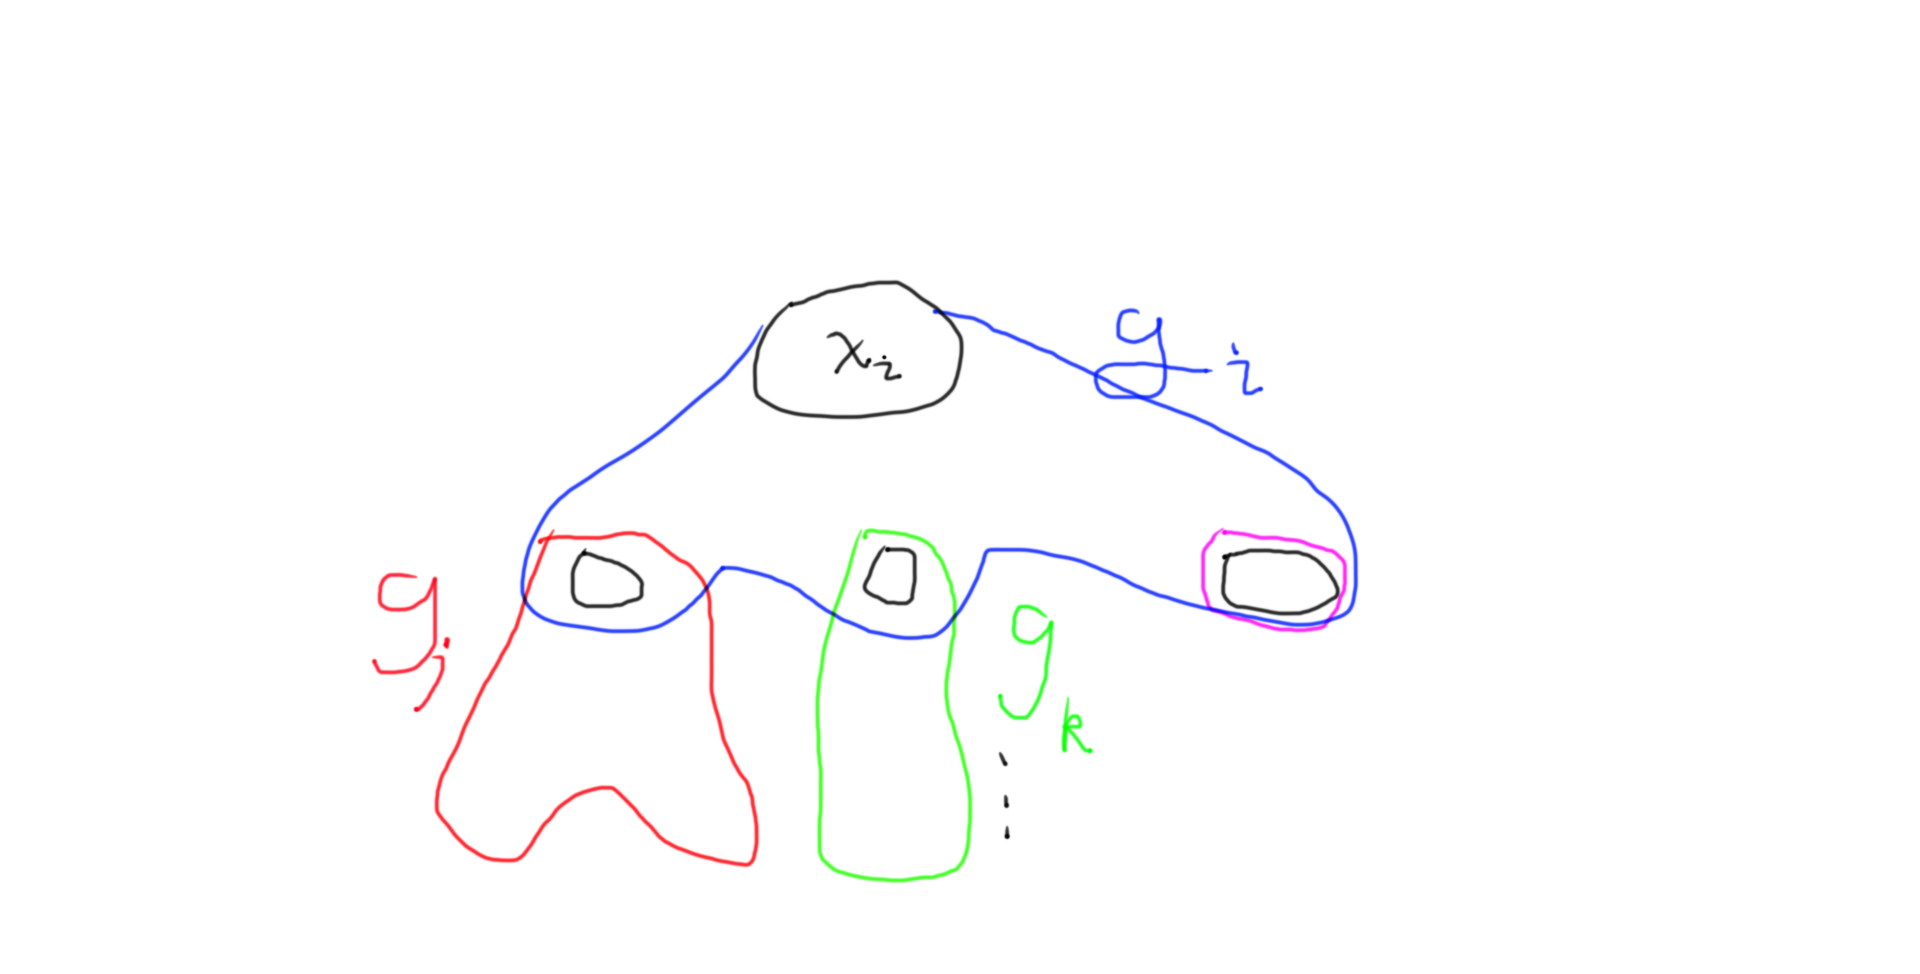
\includegraphics[width=0.70\textwidth]{comp.png}
  \end{center}
  
  如图,我们其实是给每个有根树的每个节点的儿子集合赋予了一个权值,每颗有根树的权值是每个节点的权值之乘积。
}

\subsection{点双连通子图计数}
\frame
{
  当存在 $\mathscr G$ 满足 $\mathcal G_i = \exp  \frac{\partial}{\partial x_i} \mathscr G$ 时,存在 $\mathscr F$ 使得 $\mathcal F_i = x_i \frac{\partial}{\partial x_i} \mathscr F$。我们称 $\mathscr G \mapsto \mathscr F$ 是\textbf{「点双连通-连通变换」}。(negiizhao, 2019)
  
  这里介绍一种复杂度为 $\Theta(n\Mul(n)2^n)$ 的算法,其中 $\Mul(n)$ 指代多项式乘法。(negiizhao, 2019)
}

\frame
{
  我们可以先考虑将形式稍微扩展。
  
  \begin{definition}[对称复合方程]
存在集合幂级数 $\mathscr B$,其有值项皆满足度数 $\ge 2$,和一族指数生成函数 $g_1,\dots,g_n$ 使得
$$
G_i=g_i'\circ \frac{\partial}{\partial x_i} \mathscr B
$$
时,称由 $\mathbf G$ 定义的树形复合方程是\emph{对称}的。
\end{definition}

  容易验证 $g_i = \me^x$ 的情况即为点双连通-连通变换。
}

\frame
{
  \begin{itemize}
  \item<1-> 我们考虑进行一组变换 $\mathscr B = \mathscr T_0 \rightarrow \mathscr T_1\rightarrow \dots \rightarrow \mathscr T_n = \mathscr C$。在过程中的意图为将 $g_i$ 从皆为 $x$ 逐个改为输入。因此第 $i$ 步变换会根据 $g_i$ 进行组合 $i$ 号点相邻的方点,就有
\begin{align*}
\frac{\partial}{\partial x_i} \mathscr T_{i} &= g_i \circ \frac{\partial}{\partial x_i}\mathscr T_{i-1}\\
\left.\mathscr T_i\right|_{x_i=0} &= \left.\mathscr T_{i-1}\right|_{x_i=0}
\end{align*}
  \item<2-> 每一步都可以 $\Theta(n^2 2^n)$,因此很容易做到 $\Theta(n^32^n)$。
  \end{itemize}
}

\frame
{
  \begin{itemize}
  \item<1-> 注意到中间的变换我们可以始终在插值转化的结果下进行计算,在进行第 $i$ 次变换的时候,我们只需将第 $i$ 维还原,还原一维只需要 $\Theta(n2^n)$,因此瓶颈为进行 $n$ 次在插值转化下的集合幂级数复合问题。总共复杂度为 $n\cdot \Theta(2^n\Mul(n)) = \Theta(n2^n\Mul(n))$。
  \item<2-> 这里需注意 M\"obius 变换后的复合是可以 $\Theta(2^n\Mul(n))$ 的,只需精细完成之前逐点迭代的过程。
  \end{itemize}
}

\frame
{
  \begin{itemize}
  \item<1-> 数点双子图数量的话,只需把每一步都 $\ln$ 回去就好了。
  \item<2-> 其实还有别的做法可以做到 $\Theta(n^32^n)$,但是不知道为什么很难在理论上将一个 $n^2$ 改成 $\Mul(n)$,两个做法之间的关联尚无眉目,也不能处理一般的对称复合方程,就不在这里展开了。
  \end{itemize}
}

\subsection{多变量拉格朗日反演}

\frame
{
  \begin{theorem}[多变量拉格朗日反演]
  
  对于 $H \in R((\mathbf x)), G_i \in R[[\mathbf x]]$,其中 $\mathbf x = (x_1, x_2, \dots, x_n)$。且 $G_i(0) \neq 0, F_i = x_i G_i (\mathbf F)$,其中 $\mathbf F = (F_1, F_2, \dots, F_m)$。记 $\mathbf x^{\mathbf k} = x_1^{k_1} x_2^{k_2} \cdots x_n^{k_n}$。我们有
  $$
  [\mathbf x^{\mathbf k}]H(\mathbf F) = [\mathbf x^{\mathbf k}] H \mathbf G^{\mathbf k} \left \| 
  \delta_{i,j} - \frac{x_j}{G_i(\mathbf x)} \frac{\partial G_i (\mathbf x)}{\partial x_j}
  \right \|
  $$
  \end{theorem}
  
  不难发现它在某种意义上是矩阵树定理的一个扩展形式。
}

\frame
{
  \begin{itemize}
  \item<1->我们这里给出一个结合了组合意义、以及一个矩阵中恒等式的证明。
  
  \item<2->只需证明 $H = \mathbf {x^m}$ 时的情况即可推及其线性组合,即只需证明
$$
[\mathbf x^{\mathbf k}]\mathbf {F^m} = [\mathbf x^{\mathbf k}] \mathbf {x^m}\mathbf G^{\mathbf k} \left \| 
\delta_{i,j} - \frac{x_j}{G_i(\mathbf x)} \frac{\partial G_i (\mathbf x)}{\partial x_j}
\right \|
$$

  \item<3->将其看做 EGF,则等式左侧描述的是 $m_i$ 颗以第 $i$ 种节点为根的有根树组成的森林,且第 $i$ 种节点共有 $k_i$ 个。而观察右侧,$\mathbf {x^m}\mathbf G^{\mathbf k}$ 的意图无非是先令每个节点任选其孩子集合,而这会导致一些有环的情况被统计进入,应当枚举环进行容斥。
  \end{itemize}
}

\frame
{
  \begin{itemize}
  \item<1->考虑设矩阵
$$
\mathbf M = \left(\frac{x_j}{G_i(\mathbf x)} \frac{\partial G_i (\mathbf x)}{\partial x_j}\right)_{i,j=1}^n
$$
  \item<2->那么将原图的 $t$ 个点替换为一个长度为 $t$ 的环的方法则会被 $\operatorname{tr} \mathbf M^t$ 统计 $t$ 次,故单个环进行替代的生成函数由
$$
C = \sum_{t\ge 1} \frac 1t\operatorname{tr} \mathbf M^t = \operatorname{tr}\left(\sum_{t\ge 1} \frac 1t\mathbf M^t\right) = \operatorname{tr} \left(-\log (\mathbf{I-M})\right)
$$
给出。
  \end{itemize}
}

\frame
{
  \begin{itemize}
  \item<1->故对其容斥的生成函数为 $\sum_{l\ge 0} \frac{(-C)^l}{l!}=\exp \left(-\operatorname{tr} \left(-\log (\mathbf{I-M})\right)\right) = \exp \left(\operatorname{tr} \log (\mathbf{I-M})\right)$。
  \item<2->矩阵的迹与行列式之间有关系 $\det \exp \mathbf A = \exp \operatorname{tr} \mathbf A$,带入 $\mathbf A = \log (\mathbf{I-M})$ 既得容斥因子为 $|\mathbf{I-M}|$,故命题得证。
  \item<3->对于集合幂级数而言,在实际计算时我们可以考虑计算 $\operatorname{tr} \log (\mathbf{I-M})$,这是比行列式稍微好算一点的。
  \end{itemize}
}

\frame
{
  \begin{example}[Black and White]
  已知 $f(x, y)=\frac1{1-yf(y,x)}$,求 $[x^ny^m]f(x,y)^uf(y,x)^v$。
  \end{example}
  
  \begin{itemize}
  \item<1-> 跟进过本人博客的同学可能知道,这是本人约一年前举例的生成函数输给组合意义的例证之一。
  \item<2-> 如果带入两次得到 $f=\frac{1+x-y - \sqrt{(1+x-y)^2 - 4x}}{2x}$,反而无从下手。
  \end{itemize}
}

\frame
{
  \begin{itemize}
  \item<1-> 我们不妨整理成适合多元拉格朗日反演的形式,就有 $g=xf(x,y),h=yf(y,x)$,那么可得复合方程
  \item<2-> $$\begin{cases}
g &= x \frac1{1-h}\\
h &= y \frac1{1-g}
\end{cases}$$
  \item<3-> 那么我们只需提取 $[x^{n+u}y^{m+v}]g^uh^v$,根据多元拉格朗日反演,它就等于
  \item<4-> $$
[x^ny^m]\frac1{(1-y)^{n+u}}\frac 1{(1-x)^{m+v}}\left|
\begin{matrix}
1 & -\frac y{1-y}\\
-\frac x{1-x} & 1
\end{matrix}  
\right| = {\scriptscriptstyle{\binom{n+m+v-1}n\binom{n+m+u-1}m \atop - \binom{n+m+v-1}{n-1}\binom{n+m+u-1}{m-1}}}
  $$
  \end{itemize}
}

\section{整式递推}
\frame{\sectionpage}

\frame
{
  \frametitle{整式递推}
  
  由于微分有限的生成函数之间的运算有极大的封闭性,存在一类数量不小的问题都可以通过找到整式递推式来优化计算。
  
  但大部分时候采用的方法都是一种算出前若干项之后做高斯消元(Min25 BM),在理论上还是有一点欠缺,比如不太好说明到底是几阶几次的递推式。
}

\frame
{
  接下来我们将简单介绍几个整式递推数列运算封闭性的定理与之对应的具体计算方法。这种计算方法\sout{既可以人手计算,也}可以通过计算机辅助计算。
  
  接下来的讨论中我们认为讨论一个数列 $f_n$ 符合的整式递推式与其生成函数满足的 ODE 是等价的。
}

\frame
{
  我们首先将我们常见的 GF 找出其对应的 ODE:
  
  \begin{itemize}
  \item<1-> 有限多项式:对于不超过 $d-1$ 次多项式,满足微分方程 $f^{(d)}=0$。
  
  \item<2-> 幂函数:$f=x^\alpha$ 满足微分方程 $\alpha f-xf'=0$,这里 $\alpha$ 未必是正整数,这个东西我们一般认为是复合其他 GF 时才提起。
  
  \item<3-> 广义超几何函数
  
  $$
  f = {}_p F_q(a_1,\dots a_p; b_1, \dots, b_q;x) = \sum_n \frac{a_1^{\overline n} \cdots a_p^{\overline n}}{b_1^{\overline n} \cdots b_q^{\overline n}n!}x^n
  $$
  \end{itemize}
}

\frame
{
  \frametitle{广义超几何函数微分有限}
  
  定义算子 $\vartheta = xD$,广义超几何函数满足
  
  $$
  (\vartheta + a_1) \cdots (\vartheta + a_p)f = D (\vartheta + b_1 - 1) \cdots  (\vartheta + b_q - 1)f
  $$
  
  把两边的算子展开,就是 ODE 了。
  
  这直接导出了很多函数的微分有限性:
  
  \begin{itemize}
  \item 指数函数 $\exp x = \sum_k \frac{x^k}{k!} = {}_0F_0(;;x)$
  
  \item 阶乘的 GF $\sum_k k! x^k = {}_2F_0(1,1;;x)$
  
  \item ……
  \end{itemize}
}

\subsection{封闭运算}

\frame
{
  \frametitle{加法的封闭性}
  
  假设我们已知生成函数 $f,g$ 满足的 ODE,我们希望找出一个 $f+g$ 必然满足的 ODE。我们不妨设

  $$
  f^{(n)} = \sum_{0\le k<n} p_k f^{(k)}
  $$

  其中 $p_k \in K(x)$ 即是 $K$ 上的有理分式。类似的, $g^{(m)}$ 有类似的系数 $q_k$。
}

\frame
{
  \frametitle{加法的封闭性}
  
  \begin{itemize}
  \item<1-> 接下来我们考虑如下函数列 $(f + g), (f+g)', (f+g)^{(2)},\dots$:

  \item<2-> 不妨设 $n\le m$,当 $k<n$ 的时候,$(f+g)^{(k)} = f^{(k)} + g^{(k)}$ 。而当 $k=n$ 的时候,我们注意到 $f^{(n)}$ 就可以通过我们满足的微分方程来降次了。因此我们总是可以将 $(f+g)^{(k)}$ 表示为 

  $$
  (f+g)^{(k)} = \sum_{i<n} a_i f^{(i)} + \sum_j b_jg^{(j)}
  $$
  \end{itemize}
}

\frame
{
  \frametitle{加法的封闭性}
  
  \begin{itemize}
  \item<1-> 因此我们考虑向量 $\begin{pmatrix}a_0 & \cdots & a_{n-1} & b_0 & \cdots & b_{m-1}\end{pmatrix}^{\mathsf T}$ 本来就只有 $n+m$ 个维度,因此 $(u+v)^{(0)}, \dots, (u+v)^{(n+m)}$ 必然线性相关。
  \item<2->我们只需要像维护线性基一样不断的把 $(u+v)^{(k)}$ 其被表示的向量丢进去,直到有一个向量被以前的向量线性表出即可。这也证明了 $f+g$ 满足的 ODE 的微分次数是不超过 $n+m$ 的。
  \end{itemize}
}

\frame
{
  \frametitle{乘法的封闭性}
  
  \begin{itemize}
  \item<1-> 我们类似地考虑

  $$
  (fg)^{(k)} = \sum_{i<n,j<m} a_{i,j} f^{(i)}g^{(j)}
  $$

  \item<2-> 这种表示方法在微分的时候满足 $(tf^{(i)}g^{(j)})'=t'f^{(i)}g^{(j)} + tf^{(i+1)}g^{(j)} + tf^{(i)}g^{(j+1)}$。

  \item<3-> 因此只有 $nm$ 个维度,我们类似地维护即可。
  \end{itemize}
}

\frame
{
  \begin{itemize}
    \item<1-> 这种方法的微分阶数是有明确限制的,然而其系数的多项式次数限制却不清楚是否有良好的上界。
    \item<2-> 在按照上述方法进行实际计算的时候会发生\emph{中间表示膨胀}问题,因为我们在反复求导的过程中系数有分式,而分式求导中 $\left(\frac uv\right)'=\frac{u'v-v'u}{v^2}$ 注意分母的次数是倍增的,因此在过程中分子可能会以指数级增长。
    \item<3-> 经过测试,代码在寻找 $(\ln(1-x))^3$ 的 ODE 的时候在本机花了 $3\unit{ms}$,中间通分过程最高产生过一个 $84$ 次多项式,尽管结果的多项式并不大。
  \end{itemize}
}

\subsection{复合代数幂级数}

\frame
{
  \frametitle{复合代数幂级数}
  
  \begin{itemize}
  \item<1-> 首先我们需要明确一下代数幂级数:
  \item<2-> $f$ 在 $\mathbb K[x]$ 上代数是说存在非零多项式 $G(x,y)\in \mathbb K[x,y]$ 使得 $G(x, f)=0$。
  \item<3-> 我们在实际计算的时候需通过存储 $G$ 的方式来表示这个 $f$。在解决微分有限复合代数幂级数之前我们不得不确认一下代数幂级数的四则运算如何进行。
  \end{itemize}
}

\frame
{
  \frametitle{消去平方因子}
  
  \begin{itemize}
  \item<1-> 若 $G$ 有平方因子,显然平方因子只保留一个之后,$f$ 仍是 $G$ 的一个根。
  \item<2-> 取 $G / \gcd (G, \frac{\partial}{\partial y} G)$ 即消去平方因子部分。
  \item<3-> 注意这里的 $\gcd$ 需要取 $y$ 为主元,我们不妨认为是以 $x$ 上的有理分式为系数。
  \end{itemize}
}

\frame
{
  \frametitle{倒数}
  
  注意到 $\prod_i(y-\frac 1{f_i}) = \frac1{\prod_i f_i}\prod_i (f_i y-1)$,因此我们只需将 $G$ 关于 $y$ 的系数翻转即得到 $\frac 1f$ 为一根的多项式。我们记为 $G^\rev$。
}

\frame
{
  \frametitle{和}
  
  \begin{itemize}
  \item<1-> 设 $f,g$ 分别为 $F,G$ 的根,考虑 $f+g$ 存在于哪个多项式的根。
  \item<2-> 只需考虑 $\prod_i\prod_j(y-f_i-g_j)$。结式 $\Res_z (F(x,y-z),G(x,z))$ 的性质能说明其系数是封闭的。
  \item<3-> 而具体计算其系数,可以考虑取对数:
  \begin{align*}
  &\quad \sum_i\sum_j \ln (1 - (f_i+g_j)y)\\
  &= \sum_i\sum_j \sum_{k\ge 1}  - \frac{(f_i+g_j)^k}k y^k
\end{align*}
  \end{itemize}
}

\frame
{
  \frametitle{和}
  \begin{align*}
  &= - \sum_{k\ge 1} \frac 1k y^k \sum_t \binom k t  \sum_i\sum_j  f_i^t g_j^{k-t}\\
  &= - \sum_{k\ge 1} \frac 1k y^k \sum_t \binom k t \left([y^{t-1}]\frac {\frac {\partial}{\partial y}F^{\mathsf {rev}}}{F^{\mathsf {rev}}}\right)\left([y^{k-t-1}]\frac {\frac {\partial}{\partial y}G^{\mathsf {rev}}}{G^{\mathsf {rev}}}\right)\\
  \prod_i\prod_j(1-(f_i+g_j)y) &= \exp ( \cdots )
  \end{align*}
}

\frame
{
  \frametitle{积}
  \begin{itemize}
  \item<1-> 照虎画猫,只需考虑 $\sum_i \sum_j \ln (1-f_ig_j y)$,可得其为
  \item<2-> $$ - \sum_{k\ge 1} \frac 1k y^k \left([y^{k-1}]\frac {\frac {\partial}{\partial y}F^{\mathsf {rev}}}{F^{\mathsf {rev}}}\right)\left([y^{k-1}]\frac {\frac {\partial}{\partial y}G^{\mathsf {rev}}}{G^{\mathsf {rev}}}\right) $$
  \end{itemize}
}

\frame
{
  \frametitle{微分有限复合代数幂级数}
  
  \begin{itemize}
  \item<1-> 对于一般性的 $g\in K_{\mathrm{alg}}[[x]]$ 即在 $K[x]$ 上代数的情况比较麻烦,我们不妨先考虑 $g\in K(x)$ 的情况,即有理分式。

  \item<2-> 我们考虑链式法则 $(f\circ g)' = (f'\circ g) \cdot g'$,根据分式求导法则显然 $g' \in K(x)$,我们可以得到一个下三角矩阵

  \item<3->
$$
(f\circ g)^{(k)} = \sum_{j\le k} a_{k,j} (f^{(j)} \circ g)
$$
  \end{itemize}
}

\frame
{
  \frametitle{微分有限复合代数幂级数}

  \begin{itemize}
  \item<1-> 设向量 $\mathbf v$ 的分量 $v_k$ 是 ODE 中 $f$ 的 $k$ 阶导上的系数。不难发现我们所得到的新 ODE 就是

$$
(\mathbf v \circ g) \mathbf A^{-1} \mathbf h = 0
$$

其中 $h_k = (f\circ g)^{(k)}$。

  \item<2->
我们实际上需要计算的就是 $(\mathbf v \circ g) \mathbf A^{-1}$,这个只需对增广矩阵 $[(\mathbf v \circ g) | \mathbf A]$ 做消元,把右边消成 $\mathbf I$ 的时候就得到了。注意因为是上三角矩阵,所以只需要 $\Theta(n^2)$ 次实际上是单点的行列变换。
  \end{itemize}
}

\frame
{
  \frametitle{微分有限复合代数幂级数}
  
  \begin{itemize}
  \item<1-> 接下来让我们看看一般性的情况,设 $g$ 是 $G(x,y) \in K(x)[y]$ 的根($G(x,g)=0$),设 $k$ 是 $G$ 中 $y$ 的次数。在计算复合 $h=f\circ g$ 的时候,我们希望先整理出一个带有 $g$ 的中间状态,即
  
  $$
  \sum_{j} p_j(x,g(x)) h^{(j)}(x) = 0
  $$
  
  \item<2-> 为了求出这个,我们基本可以沿用前述方法,但是这里需要注意到会对 $g(x)$ 求导,而接下来我们说明 $g'(x)$ 可以被 $g$ 表示。
  \end{itemize}
}

\frame
{
  \frametitle{微分有限复合代数幂级数}
  
  \begin{itemize}
  \item<1-> 根据 $0 = \frac{\partial}{\partial x}G(x,g)$,那么有 $g' = \frac{-(\frac{\partial}{\partial x}G)(x,g)}{(\frac{\partial}{\partial y}G)(x,g)}$。

  \item<2-> 注意我们还会反复使用到关于 $g$ 的多项式的除法,这通过与 $G(x,g)$ 的欧几里得算法可以实现,但为了保证正确性,也要求 $G(x,y)$ 关于 $y$ 在 $K(x)$ 上是\emph{不可约}的。
  \end{itemize}
}


\frame
{
  \frametitle{微分有限复合代数幂级数}
  
  \begin{itemize}
  
  \item<1-> 此时我们得到一个关于 $x,y$ 的 ODE,设其阶数为 $n$。我们将其写作
  
  $$
  h^{(n)}=\sum_{j=0}^{n-1} p_j(x,g(x)) h^{(j)}
  $$
  
  \item<2-> 考虑对此式求导,可得到一个 $h^{(n+1)}$ 与 $h^{(0)}\sim h^{(n)}$ 的关系,又可通过原式将 $h^{(n)}$ 代换掉。以此类推,我们可以得到对于 $t\ge n$,将 $h^{(t)}$ 表示为 $h^{(0)}\sim h^{(n-1)}$ 的系数,我们只关心把所有的 $y$ 消掉,而所有 $y$ 的次幂所占的维度是 $n(k-1)$,可知加入 $n(k-1)+1$ 后一定可以得到一组解,因此最终仅关于 $x$ 的 ODE 次数不超过 $nk$。
  \end{itemize}
}

\frame
{
  \begin{example}[无意识的石子堆]
  计算 $$[s^n]\frac1{\sqrt{1-s}}\mathrm{e}^{-s/2} \left(\frac{2-3s}{2-2s}\right)^{m-n}$$
  \end{example}
  
  $1$ 阶 ODE,多项式次数为 $2$。
}

\frame
{
  \begin{example}[中国象棋]
  
  计算 $$[x^n](1-x)^{-1/2} \exp\left(\frac{x(1+x)}{2-2x}\right) \frac {\left(\dfrac{2-x}{2-2x}\right)^k}{k!} \cdot
{
{}_0 F_1\left(;k+1; x\left(\frac{2-x}{2-2x}\right)^2\right)
}$$
(djq, 2020.2)
  \end{example}
  
  $8$ 阶 ODE,多项式次数为 $2$。
}

\frame
{
  \begin{example}[惠和惠惠和惠惠惠]
  
  计算 $[x^n]\left(\frac{1+x-\sqrt{1-2x-3x^2}}2\right)^m$
  \end{example}
  
  \begin{align*}
(-m(1-x-6x^2)+(1-3x-6x^2))(1+x) & F'\\
+ x(1+x)^2(1-3x)&F''\\
+ mx(-m(2+3x)+(4+3x)) &F\\
&=0
\end{align*}
}

\section{非 NTT 模数运算}
\frame{\sectionpage}

\subsection{二项基本运算}
\frame
{
  \frametitle{任意模数二项卷积}
  
  $$ h_n =\sum_k \binom nk f_kg_{n-k} $$
  
  \begin{itemize}
  \item<1-> 当模数存在 $n$ 以内的质因子时,直接转换为 EGF 是不可行的。
  
  \item<2-> 此时我们仍然有一个快速算法用于计算二项卷积,我们主要需要基于 Kummer 定理:
  \item<2-> $\binom n k$ 含有的质因子 $p$ 的次数是 $n$ 减去 $k$ 时在 $p$ 进制下退位次数。
  \end{itemize}
}

\frame
{
  \begin{itemize}
  \item<1-> 我们现在不妨设 $M=p^k$,因为一般情况总可以通过 CRT 得到。
  \item<2-> 我们记 $v_p(n)$ 是 $n!$ 中 $p$ 的质因子次数,$p$-阶乘为 $n!_p = p^{v_p(n)}$,反 $p$-阶乘为 $\overline{n!_p} = \frac{n!}{n!_p}$。

  \item<3-> 那么由定义显然 $\overline{n!_p}$ 还是同余 $M$ 可逆的。我们先令 $\widehat a_n = a_n \cdot \left( \overline{n!_p} \right)^{-1} \bmod M$,我们可以得到

$$
\widehat c_n \equiv \sum_k \left(\frac{n!_p}{k!_p (n-k)!_p}\right) \widehat a_k \widehat b_{n-k} \equiv \sum_k p^{v_p(n)-v_p(k)-v_p(n-k)} \widehat a_k \widehat b_{n-k} \pmod M
$$
  \end{itemize}
}

\frame
{
  \frametitle{“四模数 NTT”}
  \begin{itemize}
  \item<1-> $n$ 在 $p$ 进制下最多只有 $\log_p n$ 位可退,因此我们知道 $p^d \le n$,因此我们在\textbf{不取模}的情况下,可以得到 $\widehat c_n \le n \cdot nM^2 = n^2M^2$。

  \item<2-> 虽然 $p$ 在模 $M$ 下不可逆,但是当 $p\le n$,自然满足在我们选取的 NTT 模数下都可逆!
  
  \item<3->因此,这一涉及除法的卷积式子,因为已经保证了结果是值域在 $n^2M^2$ 内的整数,所以我们只需选取 NTT 模数进行卷积,之后用 CRT 合并即可。取 $n\le 10^6, M\le 10^9$ 的一般情况下,可得 $c_n \le 10^{30}$,使用四个 NTT 模数进行合并足够。
  
  (在 $n$ 稍微小一些的情况下,存在一些随机化的方法将结果值域减小到期望 $\Theta(n^{1.5}M^2)$,从而减为三个模数(lyx\_cjz, 2020.8))

  \end{itemize}
}

\frame
{
  \frametitle{其余二项运算}
  
  \begin{itemize}
  \item<1-> 求导:$a_n'=a_{n+1}$
  \item<2-> 当 $f$ 不含常数项的时候,复合运算 $g\circ f$ 是良定义的。
  \item<3-> 因为求导仍是可做的,我们可以直接迁移所有基于牛顿迭代法的算法,因此对 $f^{-1}, \ln f, \exp f$ 的运算都可以完成。
  \item<4-> 半在线二项卷积:通过四模数规约,我们将半在线二项卷积转化为四个同步进行的半在线卷积。
这在进行初等函数运算时应该也具有相当大的用处。
  \end{itemize}
}

\frame
{
  \frametitle{计算 $\frac {f^k}{k!}$}
  
  \begin{itemize}
  \item<1-> 考虑已经计算出了 $\frac{f^n}{n!}$ 与 $\frac{f^m}{m!}$,那么 $\frac{f^{n+m}}{(n+m)!}={\binom{n+m}n}^{-1} \frac{f^n}{n!}\frac{f^m}{m!}$,可以在取模 $p^k$ 的时候转为计算模 $p^{k+v_p(n+m)-v_p(n)-v_p(m)}\le(n+m)p^k$,就可以最后直接除掉 $\binom{n+m}n$。倍增即可在 $\Theta(\log k)$ 次乘法内完成。
  
  \item<2-> 这种做法可能会让原本在 \texttt{int} 范围内的取模扩大到更大的范围,额外导致了很多问题,不太好。
  \end{itemize}
}

\frame
{
  \begin{itemize}
  \item<1-> 注意到当 $n,m$ 在 $p$ 进制下加法如果不进位,则不需要扩大取模范围。我们如果能够预处理所有 $\frac{f^{p^k}}{p^k!}$,就可以在 $p$ 进制下每一位倍增,即 $\Theta(\log _p k) \cdot \Theta(\log p) = \Theta(\log k)$ 轮乘法。
   
  \item<2-> 我们又注意到,$\left(\frac{f^n}{n!}\right)' = \frac{f^{n-1}}{(n-1)!}f'$,因此我们只需在预处理的时候同步维护 $\frac{f^{p^k-1}}{(p^k-1)!}$ 即可。
  \end{itemize}
}

\section*{结尾}

\frame
{
  \begin{center}
  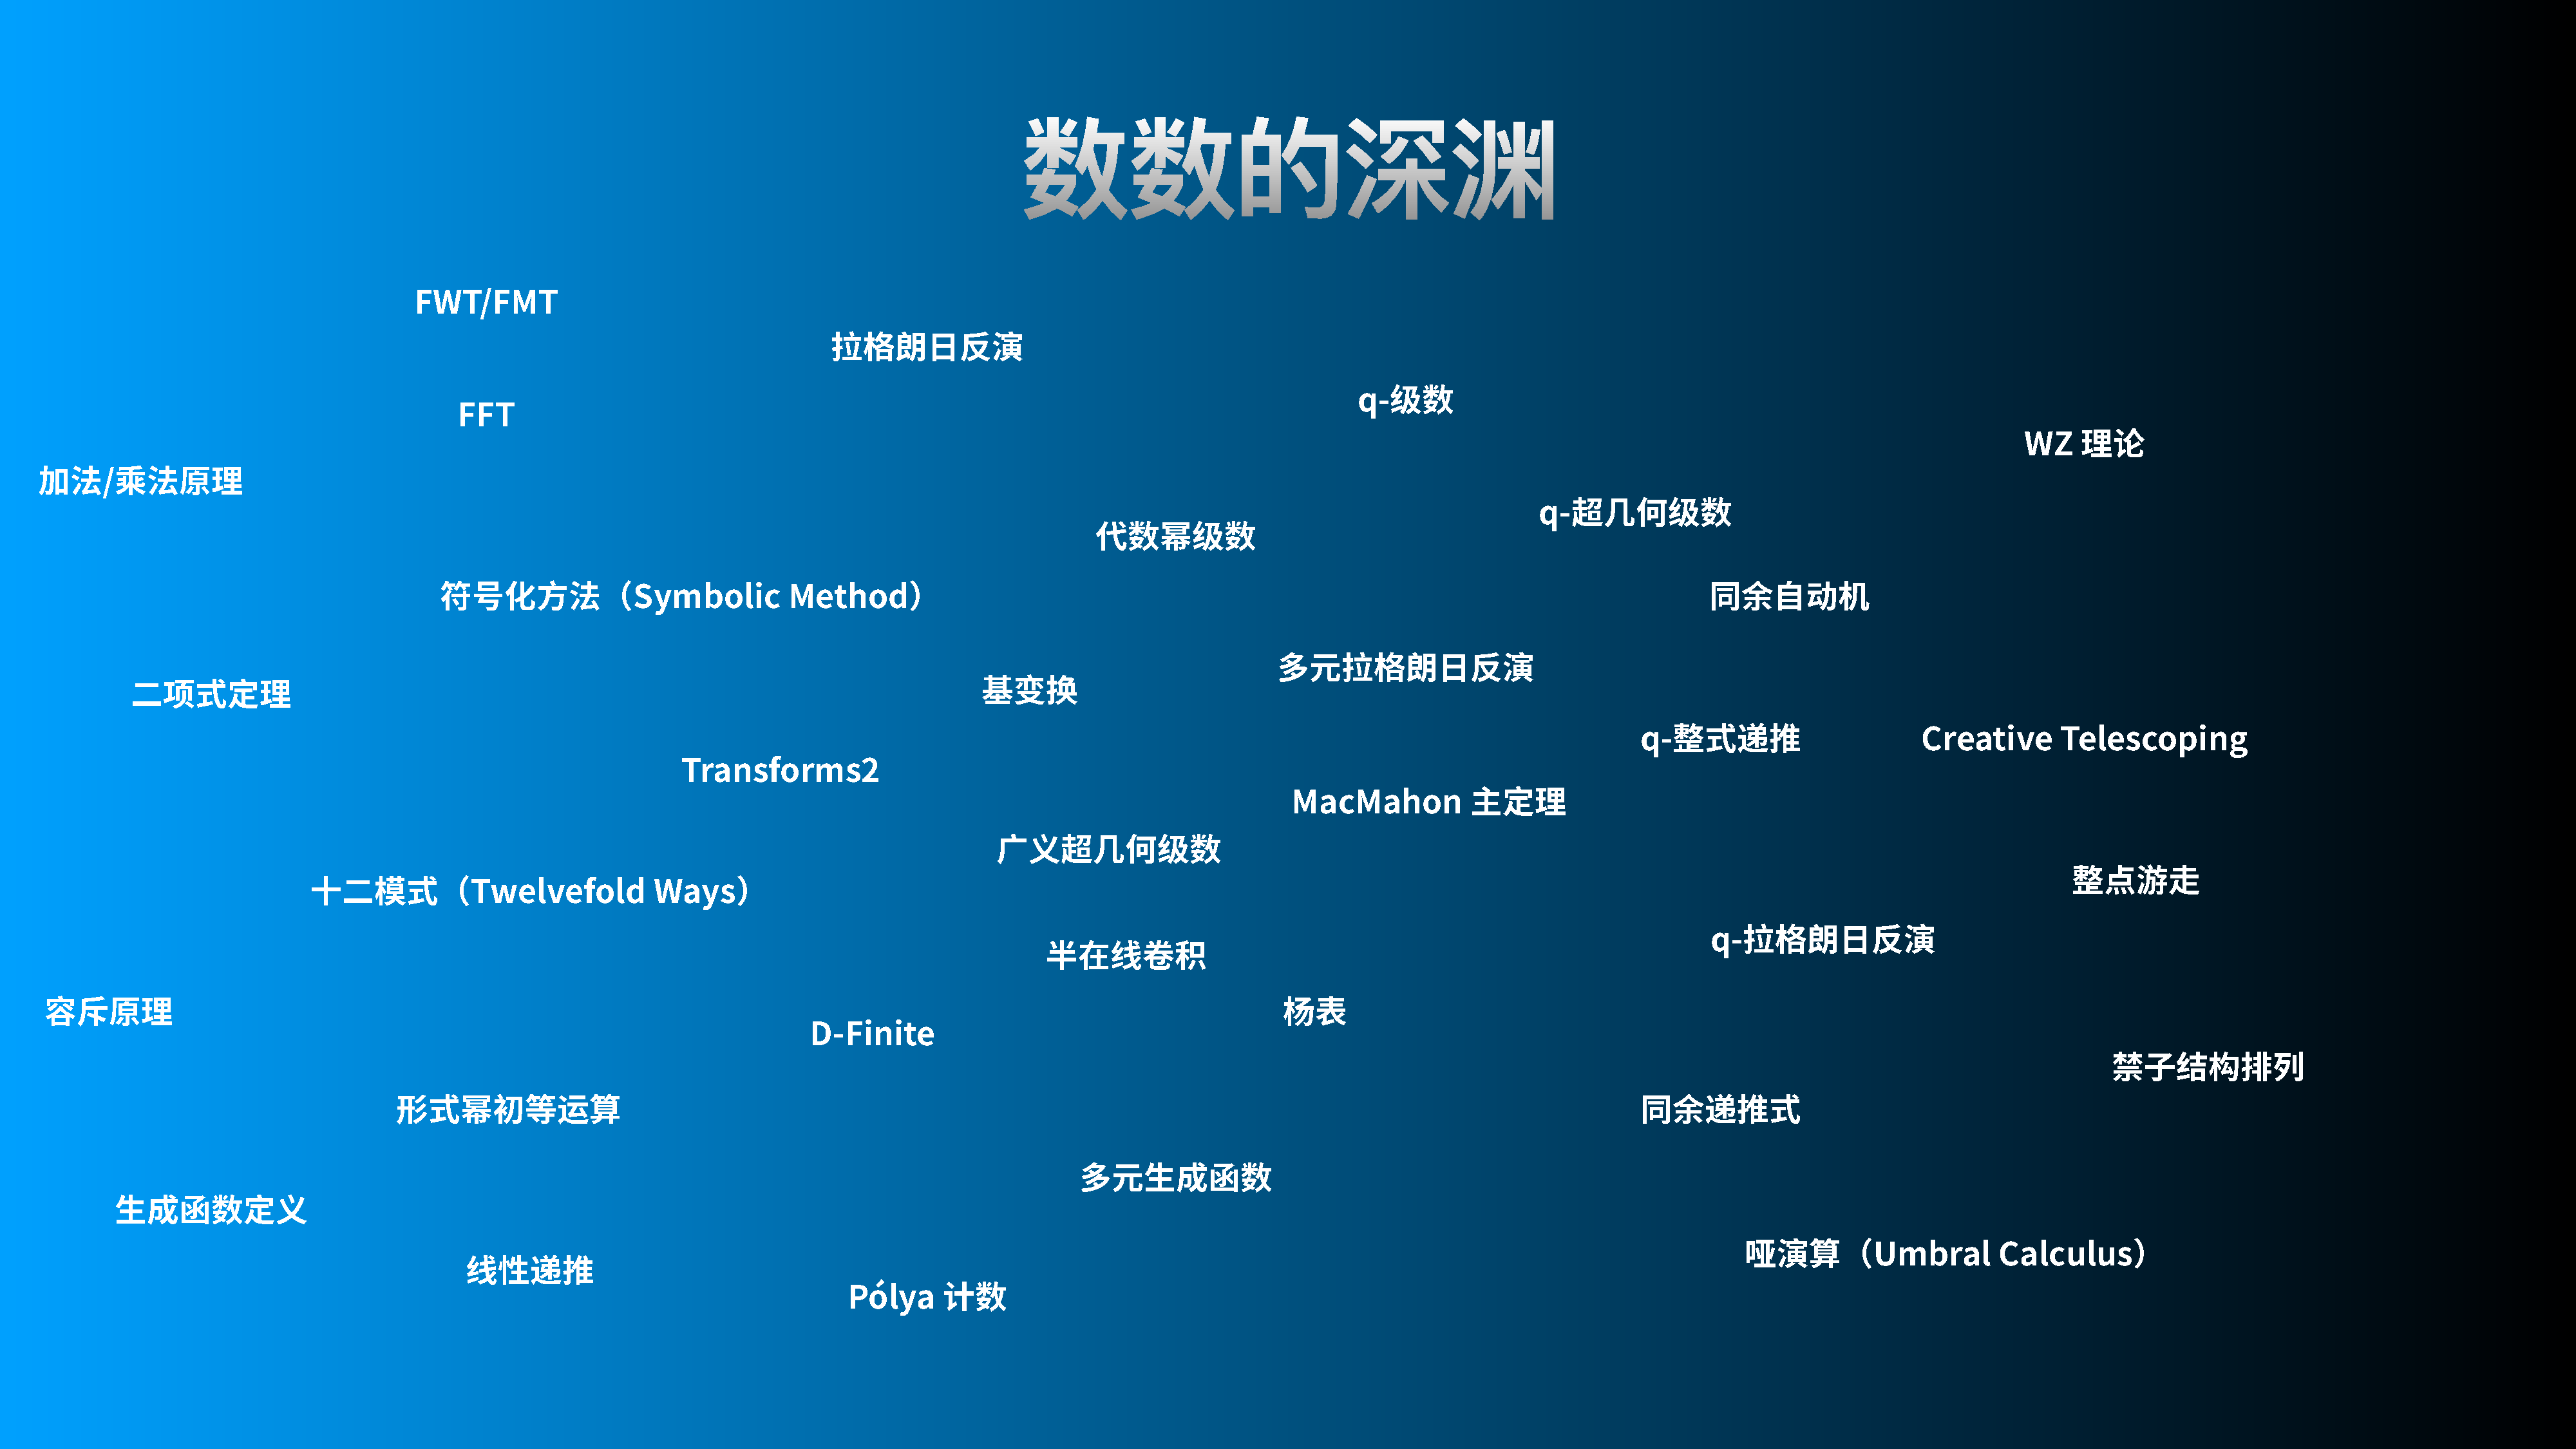
\includegraphics[width=0.70\textwidth]{deep.pdf}
  \end{center}
  
  本图仅作娱乐之用,切勿当真!
}

\frame
{
  \frametitle{谢谢大家}
  
  \begin{itemize}
  \item「宇宙很大,生活更大,也许以后还有缘相见。」\\
  \hfill ——《三体》
  \end{itemize}
}

\end{document}
